%TCIDATA{Version=5.50.0.2960}
%TCIDATA{LaTeXparent=0,0,abowd-vilhuber-PSD-2012.tex}
                      

% -*- latex -*-
%
% Time-stamp: <02/03/14 16:29:52 vilhuber>
%              Automatically adjusted if using Xemacs
%              Please adjust manually if using other editors
%
%

\subsection{The Commitment of Primary Custodians}

\begin{figure}[tbp]
\centering
\caption{The Parallel Problems of Public and Private Data Stewards}
\label{fig:accesschart}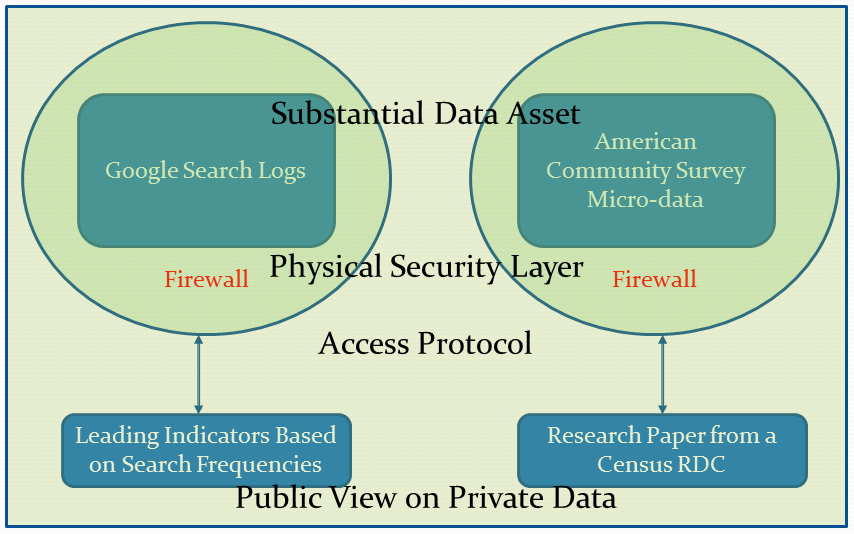
\includegraphics[width=0.5\textwidth]{accesschart}
\end{figure}

Figure \ref{fig:accesschart} shows the problem faced by public or private
data custodians who grant research access to their data. The primary data
asset is protected by both a physical security layer and an access protocol,
both of which stand between the ultimate user of the scientific output and
the confidential data. The physical security layer ensures that other
potential users do not gain unauthorized access. The access protocol limits
what may be released and published using privacy-preserving or statistical
disclosure limitation methods.

Unless the primary custodian commits to long-term archival and curation of
both the data and their metadata, the integrity of the process is corrupted.
In the private domain, future users of the published indicator cannot rely
upon the continued scrutiny of other users to expose and correct defects in
the inputs and methodology of the published indicators. In the public
domain, users of the research output cannot properly review the original
work nor reliably build on it in future work. Both failures result from the
effective denial of access to both the curated data and metadata.

Once a private or public provider commits to the long-term obligations of
scientific data custodian, the problem becomes how to integrate the archival
and curation process with their physical security layer and access
protocols. This integration is an unsolved problem although tools from both
statistical disclosure limitation and data curation are useful.

\subsection{Transparency among Users}

All of the data processing for the scientific research referenced in Figure %
\ref{fig:accesschart} is done in a controlled environment that lacks the
tools needed to conform to emerging standards for data documentation.
\textquotedblleft \lbrack T]he metadata of data files are crucial for
browsing and searching\textquotedblright\ because data files generally do
not lend themselves to the same indexing techniques as text files \cite%
{hensequadt2011}. %\marginpar{BB2 originally appeared here}
The consequence is data that are difficult to discover,
and, when found, only sparsely documented. Researchers waste valuable time
trying to determine the content and structure of confidential datasets in
sufficient detail to support their proposed secondary analysis. Some
confidential datasets even contain variables whose names themselves are
masked.\footnote{%
For example, the U.S. Census Bureau's establishment micro-data contain data
elements from the Internal Revenue Service whose confidentiality stewards
have designated the names of certain fields as \textquotedblleft official
use only,\textquotedblright\ which implies that these metadata are
confidential too.} When confronted with difficult problems such as these,
researchers resort to time-consuming alternative search strategies like
email queries.

A better solution is needed, one that allows researchers to efficiently
learn about and work with the confidential data without violating existing
access protocols, and one that ensures that the exact historical research
inputs and their provenance are curated for a long time.  Inefficiencies that
current users might be prepared to tolerate discourage potential users from
ever starting. The absence of reliable curation may effectively orphan the
research done in this early era of restricted-access data use.


\subsection{Conformance to Standards}

\begin{figure}[tbp]
\centering
\caption{Example of Confidential and Derived Public-use Metadata}
\label{fig:ConfidentialMetadata}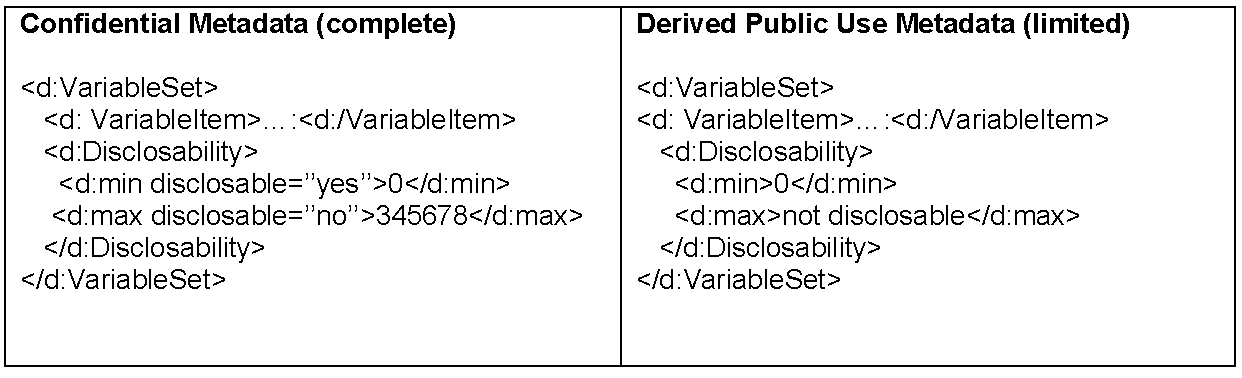
\includegraphics[width=0.5%
\textwidth]{ConfidentialMetadata}
\end{figure}

%BB2 
%\marginpar{BB2 moved here}
The Royal Society \cite{RoyalSociety2012} has recently called for metadata that goes beyond basic, generic contextual information and meets four fundamental characteristics.  Metadata must be:  accessible (a researcher can easily find it); intelligible (to various audiences); assessable (are researchers able make judgments about or assess the quality of the data); and usable (at miniumum, by other scientists). 

Leading metadata standards such as the \ac{DDI} and \ac{SDMX} are flexibly
designed to ingest documentation from a variety of source files. Using these
tools to standardize the curation of confidential research data permits the
exercise to benefit from the same technological innovations that open-access
data archives already use. \cite{GregoryHeus2007,BlankRasmussen2004}   %\marginpar{BB3}

But the benefits go in both directions. These tools need to be extended so
that they can naturally accommodate metadata items that respect
privacy-preserving and statistical disclosure limitation procedures. In a
model based on \ac{XML}, for example, this might be done through the
addition of machine-actionable attributes to elements describing variables.
An example of a possible template, assuming an \ac{XML}-like structure, is
shown in Figure \ref{fig:ConfidentialMetadata}. The example could be
applied, for instance, to a variable containing data on income or sales. The
element \textquotedblleft Disclosability\textquotedblright\ is not currently
present in the \ac{DDI} specification, but could be defined in a future
release.

The full-information metadata can be presented through a restricted-access
website available only within the secure environment itself, running the
same web frontend used for the public interface. Such a development itself
would provide a major advance in the ability of confidential data
researchers to conduct their work because in many environments, including
those supported in U.S. Census Bureau RDCs, the public metadata interface
cannot be viewed inside the secure layer and the confidential data have not
been curated to the same level of specificity.

\subsection{Training of Future Users}

Graduate social science programs and their faculties haven't worried about
how future users would gain adequate instruction in the major public-use
micro-datasets for decades. The body of discipline-specific capital is
sufficiently extensive and the data curation tools sufficiently advanced,
that doctoral programs and social science faculty members can rely on course
assignments, specialized workshops, and existing archives and repositories
to disseminate such methods. That doesn't happen with confidential data
because the potential user must usually already have a specific approved
project and be allowed access inside the security protocol layer before any
study of the metadata or analysis of the actual data can be done.

These costs are sometimes mitigated by virtual enclaves like the Cornell
VirtualRDC\footnote{%
See \href{http://www.vrdc.cornell.edu/news/}{%
http://www.vrdc.cornell.edu/news/} cited on May 20, 2012.}, the NORC\ Data
Enclave\footnote{%
See \href{http://www.dataenclave.org/index.php/home/welcome}{%
http://www.dataenclave.org/index.php/home/welcome} cited on May 20, 2012.},
or the \ac{IDSC} of the \ac{IZA}.\footnote{%
See \href{http://idsc.iza.org/}{http://idsc.iza.org/} cited on May 20, 2012}
But usually the fixed costs are simply too high to incorporate this kind of
hands-on experience in regular doctoral courses or short-term research
projects. The existence of coordinated metadata curation, as described
above, mitigates this difficulty by providing a layer of access outside of
the secure protocol for the metadata that supports the research outputs.
